\section{Forelesning 14 (Tirsdag \date{18. februar 2025})}
\subsection{Elliptic PDEs}\footnote{Section 6 B.O.}

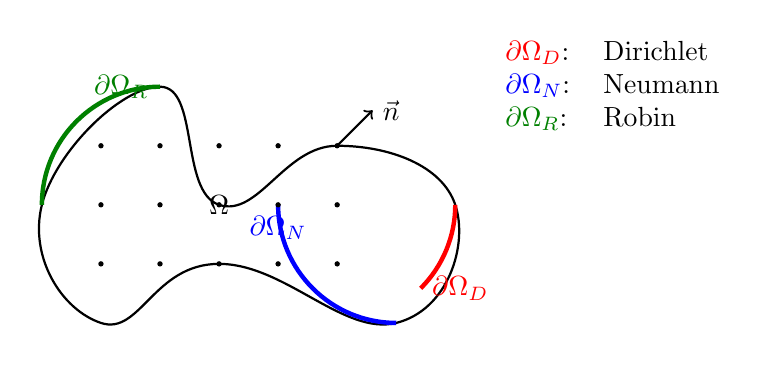
\begin{tikzpicture}[scale=1.5]
  % Draw the main omega domain with a squiggly border
  \draw[thick] plot [smooth cycle, tension=0.8] coordinates {
      (0,0) (1,0.5) (2,0) (1.5,-1) (0,-0.5) (-1,-1) (-1.5,0) (-0.5,1)
    };

  % Add colored segments for different boundary conditions
  \draw[red, ultra thick] (2,0) arc (0:-45:1) node[right] {$\partial\Omega_D$};
  \draw[blue, ultra thick] (1.5,-1) arc (-90:-180:1) node[below] {$\partial\Omega_N$};
  \draw[green!50!black, ultra thick] (-1.5,0) arc (180:90:1) node[left] {$\partial\Omega_R$};

  % Label the domain
  \node at (0,0) {$\Omega$};

  % Add normal vector demonstration
  \draw[->, thick] (1,0.5) -- (1.3,0.8) node[right] {$\vec{n}$};

  % Add grid points to show discretization
  \foreach \x in {-1,-0.5,0,0.5,1}
  \foreach \y in {-0.5,0,0.5}
  \filldraw[black] (\x,\y) circle (0.5pt);

  % Add legend
  \node[right] at (2.2,1) {
    \begin{tabular}{ll}
      \textcolor{red}{$\partial\Omega_D$}:            & Dirichlet \\
      \textcolor{blue}{$\partial\Omega_N$}:           & Neumann   \\
      \textcolor{green!50!black}{$\partial\Omega_R$}: & Robin
    \end{tabular}
  };
\end{tikzpicture}

\paragraph{Boundary Conditions}
\begin{itemize}
  \item \textbf{Dirichlet:} \(u = g\) on \(\partial\Omega_D\).
  \item \textbf{Neumann:} \(\frac{\partial u}{\partial \vec{n}} = \vec{n} \nabla u = g\) on \(\partial\Omega_N\).
  \item \textbf{Robin/Mixed:} \(\alpha u + \beta \frac{\partial u}{\partial n} = g\) on \(\partial\Omega_R\).
\end{itemize}

\[
  \partial \Omega = \overline{\partial \Omega_D \cup \partial \Omega_N \cup \partial \Omega_R}
\]

\begin{enumerate}
  \item Find a \emph{FDS} for the model problem.
  \item Implement and test the method.
  \item Error analysis.
  \item How to deal with less nice boundaries and irregular grids.
\end{enumerate}

\subparagraph{Model Problem}
\[
  \begin{cases}
    u_{xx} + u_{yy} = f(x,y) & \text{on} \quad \Omega = (0,1) \times (0,1)                                \\
    u = g                    & \text{on} \quad \partial \Omega_D (x = 0 \lor x = 1 \lor y = 0 \lor y = 1) \\
  \end{cases}
\]

\begin{enumerate}
  \item \emph{FDS:} Discretize the domain \(\Omega\) and the boundary \(\partial \Omega_D\).
        \begin{align*}
          \Omega_h              & = \{(x_i, y_j) \mid x_i = ih, y_j = jh, i,j = 0,1,\ldots,N\} \\
          \partial \Omega_{D,h} & = \{(x_i, y_j) \mid x_i = ih, y_j = jh, i,j = 0,1,\ldots,N\} \\
          \mathring{\Omega}_h   & = \Omega_h \setminus \partial \Omega_{D,h}
        \end{align*}
  \item \emph{Test:} Implement and test the method.
        \begin{align*}
          u_{xx}(x_i, y_j) & \approx \frac{1}{h^2}(u_{i+1,j} - 2u_{i,j} + u_{i-1,j}) + \frac{h^2}{6}\partial_x^4 u(x_i, y_j) \\
          u_{yy}(x_i, y_j) & \approx \frac{1}{h^2}(u_{i,j+1} - 2u_{i,j} + u_{i,j-1}) + \frac{h^2}{6}\partial_y^4 u(x_i, y_j)
        \end{align*}
  \item Let \(u_{i,j} = u(x_i, y_j)\) and \(f_{i,j} = f(x_i, y_j)\), with Numerical Solution \(U_{i,j} \approx u_{i,j}\).
        \[
          \frac{1}{h^2}\left(U_{i+1,j} + U_{i,j+1} - 4U_{i,j} + U_{i-1,j} + U_{i,j-1}\right) = f_{i,j}
        \]
  \item \emph{Computional Stencil:}
        \begin{align*}
          P = (x_i, y_j) \quad \text{and} \quad E = (x_{i+1}, y_j) \quad \text{and} \quad N = (x_i, y_{j+1})     \\
          W = (x_{i-1}, y_j) \quad \text{and} \quad S = (x_i, y_{j-1})                                           \\
          U_{i,j} = \frac{1}{4}\left(U_{i+1,j} + U_{i,j+1} + U_{i-1,j} + U_{i,j-1}\right) - \frac{h^2}{4}f_{i,j} \\
          U_N + U_E + U_W + U_S - 4U_P = h^2 f_P \quad P \in \mathring{\Omega}_h
        \end{align*}
  \item \emph{Error Analysis:} Estimate the error.
\end{enumerate}
\begin{definition}{Natural Ordering}{}
  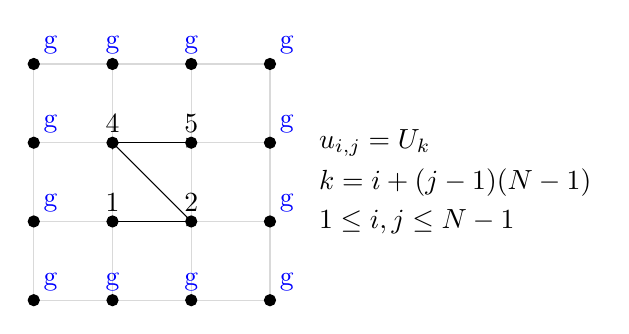
\begin{tikzpicture}
    % Grid
    \draw[step=1cm,gray!30] (0,0) grid (3,3);

    % Node points with numbers showing ordering
    \foreach \x in {0,1,2,3}
    \foreach \y in {0,1,2,3} {
        \filldraw[black] (\x,\y) circle (2pt);
      }

    % Natural ordering labels
    \node[above] at (1,1) {1};
    \node[above] at (2,1) {2};
    \node[above] at (1,2) {4};
    \node[above] at (2,2) {5};

    % Boundary points marked with g
    \foreach \x in {0,3}
    \foreach \y in {0,...,3} {
        \node[blue, above right] at (\x,\y) {g};
      }
    \foreach \x in {1,2}
    \foreach \y in {0,3} {
        \node[blue, above] at (\x,\y) {g};
      }

    % Arrows showing ordering direction
    \draw[->] (1,1) -- (2,1);
    \draw[->] (2,1) -- (1,2);
    \draw[->] (1,2) -- (2,2);

    % Equation labels
    \node[right] at (3.5,2) {$u_{i,j} = U_k$};
    \node[right] at (3.5,1.5) {$k = i + (j-1)(N-1)$};
    \node[right] at (3.5,1) {$1 \leq i,j \leq N-1$};
  \end{tikzpicture}
  \begin{align*}
    \frac{1}{h^2}
    \begin{bmatrix}
      -4     & 1      & 0      & \cdots & 0      & 1      & 0      & \cdots & 0      \\
      1      & -4     & 1      & \cdots & 0      & 0      & 1      & \cdots & 0      \\
      0      & 1      & -4     & \cdots & 0      & 0      & 0      & \cdots & 0      \\
      \vdots & \vdots & \vdots & \ddots & \vdots & \vdots & \vdots & \ddots & \vdots \\
      1      & 0      & 0      & \cdots & -4     & 1      & 0      & \cdots & 0      \\
      0      & 1      & 0      & \cdots & 1      & -4     & 1      & \cdots & 0      \\
      \vdots & \vdots & \vdots & \ddots & \vdots & \vdots & \vdots & \ddots & \vdots \\
      0      & 0      & 0      & \cdots & 0      & 1      & 0      & \cdots & -4
    \end{bmatrix}
    \begin{bmatrix}
      U_{1,1} \\
      U_{2,1} \\
      U_{3,1} \\
      \vdots  \\
      U_{1,2} \\
      U_{2,2} \\
      \vdots  \\
      U_{N,N}
    \end{bmatrix}
    =
    \begin{bmatrix}
      f_{1,1} - \frac{1}{h^2}(g_W + g_S) \\
      f_{2,1} - \frac{1}{h^2}g_S         \\
      f_{3,1} - \frac{1}{h^2}g_S         \\
      \vdots                             \\
      f_{1,2} - \frac{1}{h^2}g_W         \\
      f_{2,2}                            \\
      \vdots                             \\
      f_{N,N} - \frac{1}{h^2}(g_E + g_N)
    \end{bmatrix}
  \end{align*}
\end{definition}

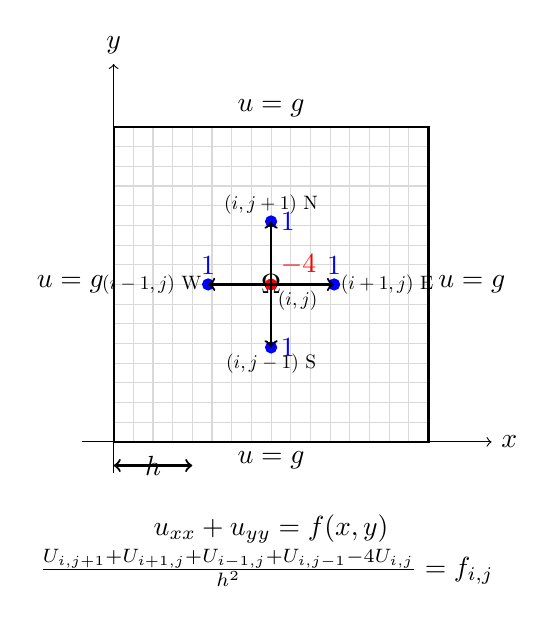
\begin{tikzpicture}[scale=1]
  % Grid
  \draw[step=0.25,gray!30] (0,0) grid (4,4);

  % Domain boundary
  \draw[thick] (0,0) rectangle (4,4);

  % Axes
  \draw[->] (-0.4,0) -- (4.8,0) node[right] {$x$};
  \draw[->] (0,-0.4) -- (0,4.8) node[above] {$y$};

  % Label domain
  \node at (2,2) {$\Omega$};

  % Label boundary conditions
  \node[left] at (0,2) {$u=g$};
  \node[right] at (4,2) {$u=g$};
  \node[below] at (2,0) {$u=g$};
  \node[above] at (2,4) {$u=g$};

  % Grid points for computational stencil (centered at 2,2)
  \filldraw[red] (2,2) circle (2pt) node[below right,black,scale=0.7] {$(i,j)$};
  \filldraw[blue] (2.8,2) circle (2pt) node[right,black,scale=0.7] {$(i+1,j)$ E};
  \filldraw[blue] (2,2.8) circle (2pt) node[above,black,scale=0.7] {$(i,j+1)$ N};
  \filldraw[blue] (1.2,2) circle (2pt) node[left,black,scale=0.7] {$(i-1,j)$ W};
  \filldraw[blue] (2,1.2) circle (2pt) node[below,black,scale=0.7] {$(i,j-1)$ S};

  % Arrows showing relationships 
  \draw[->,thick] (2,2) -- (2.8,2);
  \draw[->,thick] (2,2) -- (2,2.8);
  \draw[->,thick] (2,2) -- (1.2,2);
  \draw[->,thick] (2,2) -- (2,1.2);

  % Equation labels
  \node[below] at (2,-0.8) {$u_{xx} + u_{yy} = f(x,y)$};

  % Add coefficient labels
  \node[red] at (2,2) [above right] {$-4$};
  \node[blue] at (2.8,2) [above] {$1$};
  \node[blue] at (2,2.8) [right] {$1$};
  \node[blue] at (1.2,2) [above] {$1$};
  \node[blue] at (2,1.2) [right] {$1$};

  % Add mesh size label
  \draw[<->, thick] (0,-0.3) -- (1,-0.3);
  \node at (0.5,-0.3) {$h$};

  % Add computational stencil formula
  \node[align=center] at (2,-1.6) {
    $\frac{U_{i,j+1} + U_{i+1,j} + U_{i-1,j} + U_{i,j-1} - 4U_{i,j}}{h^2} = f_{i,j}$
  };
\end{tikzpicture}


\begin{align*}
  \symbf{A} & =
  \begin{bmatrix}
    B      & I      & 0      & \cdots & 0      & 0      & 0      & \cdots & 0      \\
    I      & B      & I      & \cdots & 0      & 0      & 0      & \cdots & 0      \\
    0      & I      & B      & \cdots & 0      & 0      & 0      & \cdots & 0      \\
    \vdots & \vdots & \vdots & \ddots & \vdots & \vdots & \vdots & \ddots & \vdots \\
    0      & 0      & 0      & \cdots & B      & I      & 0      & \cdots & 0      \\
    0      & 0      & 0      & \cdots & I      & B      & I      & \cdots & 0      \\
    0      & 0      & 0      & \cdots & 0      & I      & B      & \cdots & 0      \\
  \end{bmatrix}
  = \operatorname{blocktridiag}(B,I,I) \in \mathbb{R}^{(M-1)^2 \times (M-1)^2} \\
  \text{where} \quad
  \symbf{B} & = \begin{bmatrix}
                  -4     & 1      & 0      & \cdots & 0      \\
                  1      & -4     & 1      & \cdots & 0      \\
                  0      & 1      & -4     & \cdots & 0      \\
                  \vdots & \vdots & \vdots & \ddots & \vdots \\
                  0      & 0      & 0      & \cdots & -4
                \end{bmatrix}
  = \operatorname{tridiag}(1,-4,1) \in \mathbb{R}^{(M-1)\times(M-1)}
\end{align*}

\(\symbf{A}\) is very large. if \(M=100\) then \(\symbf{A} \in \mathbb{R}^{9801 \times 9801}\).

But \(\symbf{A}\) is \emph{sparse} and \emph{banded}.

\begin{definition}{5-point formula}{}
  The 5-point formula for discretizing the Poisson equation is:

  \begin{equation*}
    U_{i,j} = \frac{1}{4}\left(U_{i+1,j} + U_{i,j+1} + U_{i-1,j} + U_{i,j-1}\right) - \frac{h^2}{4}f_{i,j}
  \end{equation*}

  This formula relates each interior grid point to its four nearest neighbors, giving it an error of $O(h^2)$ where $h$ is the grid spacing.
\end{definition}
